\section{Efficient architecture}

For building an efficient training architecture, we start by answering the following questions:

\begin{itemize}
    \item What is the family of algorithms that should be supported by this architecture? --- In
    this paper we are aiming to provide a training architecture that will cover model-free
    off-policy and on-policy algorithms with bounded staleness of samples.

    \item What hardware will be used to run the algorithm? --- We consider hybrid CPU/GPU system,
    as it's currently the most widely used platform for training neural networks, and also because
    it provides a good balance between sampling and training performance.

    \item What are the bottlenecks that prevent current algorithms to perform well? --- Most of the
    current algorithms introduce sequential dependency between acting and training procedure, that
    is absolutely unnecessary and prevents from fully utilizing a hardware and also leads to the
    slowdown when there is a skew in components performance.
\end{itemize}

We end up with the architecture that consists of the following components:
\begin{itemize}
    \item Actor --- interacts with the environment, by acting and collection the experience. To
        make actions. Uses a separate model replica that is periodically synced with the master replica.
        Runs on CPU, as it doesn't require parallelism or low-latency. Can be scaled up to several
        instances to address slow environment problem.

    \item Trainer --- collects the experience produced by actors and decides which samples will be
        used by learner to train the model. This might include using an internal experience replay
        table or just filtering old samples and forwarding them to the learner.

    \item Learner --- consumes samples provided by trainer to compute gradients and update the
        master model. Runs on GPU, as it needs to perform heavy batch computations.
\end{itemize}

\begin{figure}[h!]
\caption{Training architecture}
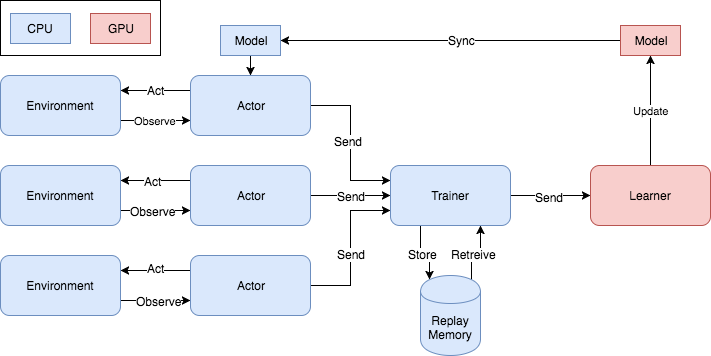
\includegraphics[width=\textwidth]{architecture}
\end{figure}

\begin{algorithm}
    \caption{Actor thread}\label{actor}
    \begin{algorithmic}[1]
        \State $env \gets MakeEnv(seed)$
        \State $state \gets env.Start()$
        \State $T \gets 0$
        \While{TrainingNotDone}
            \If{$T \mod F_{sync} = 0$}
                \State $model \gets SyncModel()$
            \EndIf
            \State $action \gets model.Predict(state)$
            \State $nextState, reward \gets env.Act(action)$
            \State $actorQueue.Enqueue(state, action, reward, nextState)$
            \State $state \gets nextState$
            \State $T \gets T + 1$
        \EndWhile
    \end{algorithmic}
\end{algorithm}

\begin{algorithm}
    \caption{Trainer thread}\label{trainer}
    \begin{algorithmic}[1]
        \While{TrainingNotDone}
            \State $states, actions, rewards, nextStates \gets actorQueue.Dequeue()$
            \State $StoreExperience(states, actions, rewards, nextStates)$
            \State $learnerQueue.Enqueue(SampleExperience(batchSize))$
        \EndWhile
    \end{algorithmic}
\end{algorithm}

\begin{algorithm}
    \caption{Learner thread}\label{learner}
    \begin{algorithmic}[1]
        \For{$T \gets 0, T_{max}$}
            \State $batch \gets learnerQueue.Dequeue()$
            \State $Train(batch)$
        \EndFor
    \end{algorithmic}
\end{algorithm}

- Description of more efficient architecture, and questions that we need to
  answer to build it. Compare with PAAC, GA3C, tell when one is better then
  the other and vice versa.

In this section we describe:
- Tell that this is our new ideas.

- Tell how it looks like. Simple description of the process in terms of multiple CPU and 1 GPU.

- Give a code for actor, trainer and learner.

- Tell how this compares to other architectures, in what regimes it should operate better then
the other algorithms.

- Tell about resulting GPU utilization and time spent in different modes of operation.

- Tell about existing bottlenecks, what will be the limiting factor depending on the env speed,
training speed, network size.

- Tell how this is applicable to DQN and ACER (and any algorithm with experience replay, or
slightly off-policy data tolerance).
